\documentclass{exam}
\usepackage[utf8]{inputenc}
\usepackage{lmodern}
\usepackage{microtype}

% \usepackage[parfill]{parskip}
\usepackage[dvipsnames]{xcolor}
\usepackage{amsmath}
\usepackage{amsfonts}
\usepackage{amsthm}
\usepackage{siunitx}
\DeclareSIUnit\year{yr}
\DeclareSIUnit\foot{ft}
\DeclareSIUnit\litre{\liter}

\usepackage{skull}

\usepackage{pgfplots}
\usepgfplotslibrary{polar}
\pgfplotsset{compat=1.11}
\usepgfplotslibrary{statistics}
\usepackage{graphicx}
\usepackage{sidecap}
\sidecaptionvpos{figure}{c}
\usepackage{float}
\usepackage{gensymb}
\usepackage{tkz-euclide}
\usetkzobj{all}
\usepackage{commath}
\usepackage{hyperref}
\usepackage{enumitem}
\usepackage{wasysym}
\usepackage{multicol}
\usepackage{mathtools}
\usepackage{tcolorbox}
\usepackage{tabularx}
\usepackage[version=4]{mhchem}
\usepackage{changepage}
\usepackage{listings}
\lstset{basicstyle=\ttfamily\linespread{0.8}\small}

\renewcommand*{\thefootnote}{\fnsymbol{footnote}}

\newtheorem*{thm}{Theorem}
\newtheorem*{iden}{Identity}
\newtheorem*{lemma}{Lemma}
\newtheorem{obs}{Observation}
\theoremstyle{definition}
\newtheorem*{defn}{Definition}
\newtheorem*{ex}{Example}
\newtheorem{con}{Construction}
\newtheorem*{alg}{Algorithm}

\newtheoremstyle{break}
  {\topsep}{\topsep}%
  {\itshape}{}%
  {\bfseries}{}%
  {\newline}{}%
\theoremstyle{break}
\newtheorem*{bthm}{Theorem}

% russian integral
\usepackage{scalerel}
\DeclareMathOperator*{\rint}{\scalerel*{\rotatebox{17}{$\!\int\!$}}{\int}}

% \DeclareMathOperator*{\rint}{\int}

\pgfplotsset{vasymptote/.style={
    before end axis/.append code={
        \draw[densely dashed] ({rel axis cs:0,0} -| {axis cs:#1,0})
        -- ({rel axis cs:0,1} -| {axis cs:#1,0});
    }
}}

% \pointsinrightmargin
\boxedpoints
\pointname{}

\newcommand{\questioA}{\question[\texttt{\textbf{\color{Cerulean} A}}]}
\newcommand{\questioM}{\question[\texttt{\textbf{\color{PineGreen} M}}]}
\newcommand{\questioE}{\question[\texttt{\textbf{\color{WildStrawberry} E}}]}
\newcommand{\questioS}{\question[\texttt{\textbf{\color{Goldenrod} S}}]}
\newcommand{\questioO}{\question[\texttt{\textbf{\color{BurntOrange} O}}]}

\newcommand{\parA}{\part[\texttt{\textbf{\color{Cerulean} A}}]}
\newcommand{\parM}{\part[\texttt{\textbf{\color{PineGreen} M}}]}
\newcommand{\parE}{\part[\texttt{\textbf{\color{WildStrawberry} E}}]}
\newcommand{\parS}{\part[\texttt{\textbf{\color{Goldenrod} S}}]}
\newcommand{\parO}{\part[\texttt{\textbf{\color{BurntOrange} O}}]}

\newcommand{\subparA}{\subpart[\texttt{\textbf{\color{Cerulean} A}}]}
\newcommand{\subparM}{\subpart[\texttt{\textbf{\color{PineGreen} M}}]}
\newcommand{\subparE}{\subpart[\texttt{\textbf{\color{WildStrawberry} E}}]}
\newcommand{\subparS}{\subpart[\texttt{\textbf{\color{Goldenrod} S}}]}
\newcommand{\subparO}{\subpart[\texttt{\textbf{\color{BurntOrange} O}}]}

\newcommand{\mainHeader}[2]{\section*{NCEA Level 2 Mathematics\\#1. #2}}
\newcommand{\mainHeaderHw}[2]{\section*{NCEA Level 2 Mathematics (Homework)\\#1. #2}}
\newcommand{\seealso}[1]{\begin{center}\emph{See also #1.}\end{center}}
\newcommand{\drills}[1]{\begin{center}\emph{Drill problems: #1.}\end{center}}
\newcommand{\basedon}[1]{\begin{center}\emph{Notes largely based on #1.}\end{center}}


\begin{document}

\mainHeader{2}{Arcs and Sectors of Circles}
The Greeks studied two fundamental geometric objects: lines, and circles. Last week we looked at lines; this time, we will look at
circles.

A circle is simply the set of all points that are at a distance $ r $ from a point $ (x_0, y_0) $: the point $ (x_0,y_0) $ is called
the centre of the circle, and the distance $ r $ is the radius of the circle. If $ (x,y) $ is a point on the circle, then we have
\begin{displaymath}
  d((x,y), (x_0,y_0)) = r \implies \sqrt{(x - x_0)^2 - (y - y_0)^2} = r
\end{displaymath}
and the equation of the circle in cartesian coordinates is $ (x - x_0)^2 + (y - y_0)^2 = r^2 $.

\subsection*{Circumferii}
\begin{center}
  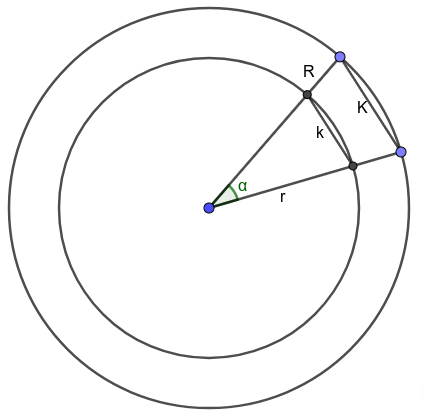
\includegraphics[width=0.4\textwidth]{pi}
\end{center}

Suppose the angle $ \alpha $ is measured in degrees. Then the circumference of the inner circle is $ c \approx \frac{\ang{360}}{\alpha} k $,
and the circumference of the outer circle is $ C \approx \frac{\ang{360}}{\alpha} K $. Now, the two triangles formed are similar since
they have an identical angle and two sides with the same ratio of $ r/R $; hence $ k/K = r/R $. We can rewrite:
\begin{displaymath}
  \frac{k}{K} = \frac{r}{R} \implies \frac{c \frac{\alpha}{\ang{360}}}{C \frac{\alpha}{\ang{360}}} \approx \frac{r}{R} \implies \frac{c}{C} \approx \frac{r}{R}.
\end{displaymath}
As the size of the angle $ \alpha $ becomes smaller and smaller, this approximation becomes exact: $ \frac{c}{C} = \frac{r}{R} $, and
so $ \frac{c}{r} = \frac{C}{R} $. In other words, the ratio of the circumference of any circle to its radius is always the same. For historical
reasons, we actually write this in terms of the diameter, and call the constant of proportionality $ \pi $. We have therefore sketched a
proof that
\begin{displaymath}
  c = 2\pi r
\end{displaymath}
for any circle with radius $ r $ and circumference $ c $.

The number $ \pi $ is approximately equal to
\begin{displaymath}
  3.1415926535897932384626433...
\end{displaymath}
and in one of the exercises below you will calculate a first approximation to this value: it isn't just
a number that is plucked out of thin air!

\subsection*{Areas}
The other main result we have for circles is the area; by slicing the circle into smaller and smaller pieces, we can
approximate the area of a circle with the area of a rectangle:
\begin{center}
  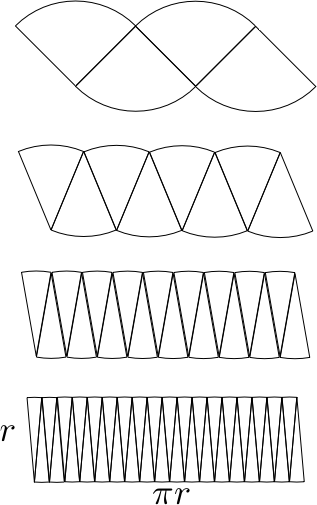
\includegraphics[width=0.25\textwidth]{area}
\end{center}
By means of this, we can intuitively justify that the area of a circle with radius $ r $ is
\begin{displaymath}
  A = \pi r^2.
\end{displaymath}

This idea of a limiting process will be made more clear next year (when you will be able to provide proper proofs of
these facts), but hopefully these two results seem plausible.

\subsection*{Thale's Theorem}
As a taster for some of the other pretty theorems one can prove about circles, consider any circle; pick a diameter of the
circle and any point on the circle itself; then the resulting triangle is always right-angled, as in the following diagram.
\begin{center}
  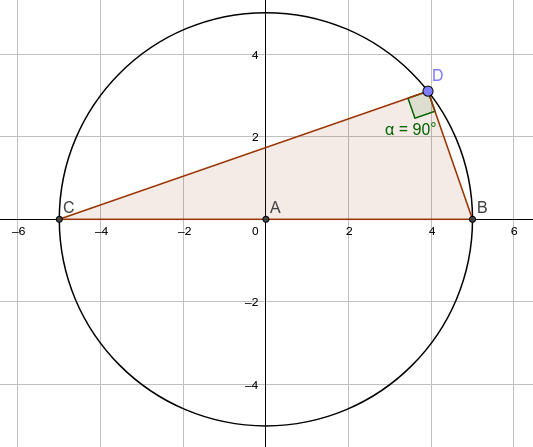
\includegraphics[width=0.5\textwidth]{thales}
\end{center}

I actually know \emph{two} proofs of this; we'll look at both!

\begin{proof}[Angle-y proof]
  The first proof is quite cute: we simply consider the next figure and do some angle pushing.
  \begin{center}
    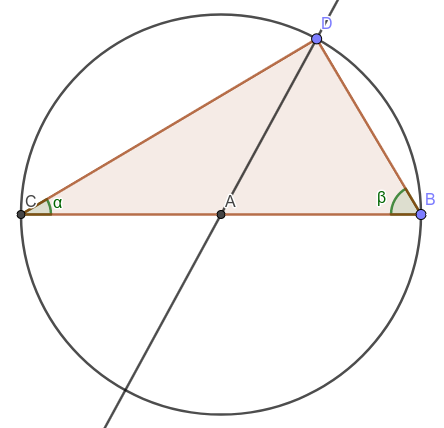
\includegraphics[width=0.4\textwidth]{thales2}
  \end{center}
  Clearly $ ACD $ and $ ABD $ are both isosceles, so $ CDA = \alpha $ and $ ADB = \beta $; hence $ CDB = \alpha + \beta $,
  and so (using the fact that the internal angles of a triangle add to \ang{180}) we have $ \ang{180} = \alpha + \beta + \alpha + \beta $;
  so $ CDB = \alpha + \beta = \ang{180}/2 = \ang{90} $.
\end{proof}

\begin{proof}[Rotate-y proof]
  The intuitive idea behind the second proof is that we take the triangle, `rotate it around', and see that the resulting shape is a rectangle.
  In order to make this idea more precise, consider the following diagram.
  \begin{center}
    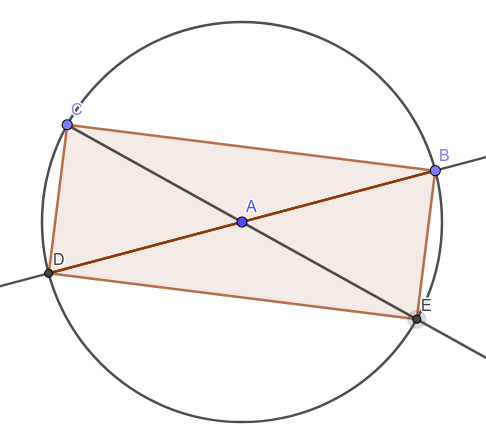
\includegraphics[width=0.4\textwidth]{thalesrotate}
  \end{center}
  Here, we took our initial triangle to be $ BCD $, sitting on the diameter $ BD $. Draw the line through $ C $ and $ A $; clearly (since it
  passes through the centre) it is a diameter of the circle. Hence the two diagonals of the quadrilateral $ BCDE $ are the same length,
  and it is therefore a rectangle (so in particular $ DCB $ is a right angle).
\end{proof}

Which proof do you prefer? Why?

\clearpage
\subsection*{Questions}
\begin{questions}
  \question Suppose we take a circle of radius $ r $, and cut out a slice with an angle $ \alpha $ (like cutting a pizza). Draw a picture.
            What is the area of this slice, and what is the length of the arc of the circumference that is part of the slice?
            (Such a slice is called a \textit{sector}.)
  \question Notice that the formulae derived above all have ugly factors of \ang{360}. Define one radian to be the angle such that the
            arc length of the sector defined by that angle is just $ r $, the radius of the circle. Radians are, in many ways, a much
            more natural angle measurement unit.
    \begin{parts}
      \part Draw a picture to show this geometrically.
      \part Show that one radian is precisely $ \frac{\pi}{180} $ degrees.
      \part How many radians are in a full circle?
      \part Show that, in radians, the formulae derived in question 1 above simplify dramatically.
    \end{parts}
  \question Suppose a circle has area $ 49\pi $. What is the arc length of a sector of this circle with area $ 25\pi $?
  \question Show that if the angle subtended by a chord at the centre is \ang{90} then $ \ell = \sqrt{2}r $, where $ \ell $
            is the length of the chord.
  \question In the following diagram, the two circles are centred at $ A $ and $ B $ and intersect at $ C $ and $ D $. The
            quadrilateral $ ABCD $ is a square. Consider the shaded area as a subset of one of the circles. What proportion
            of the circle's area is shaded?
            \begin{center}
              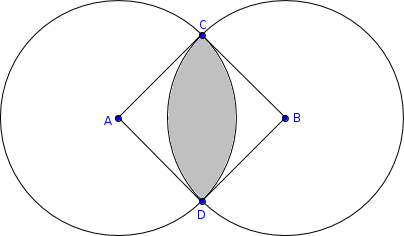
\includegraphics[width=0.5\textwidth]{overlapcircle}
            \end{center}
  \question Suppose that two lines tangent to a circle at points $ B $ and $ C $ intersect at a point $ D $, as shown. Show that
            the two segments $ BD $ and $ CD $ have equal lengths. \label{exercise:tangents}
            \begin{center}
              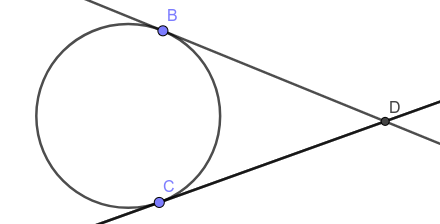
\includegraphics[width=0.4\textwidth]{cirtangents}
            \end{center}
  \question A simple definition of a circle is the set of all points $ P = (x,y) $ such that $ d(A, P) = r $ (where $ A $ is the centre of the circle
            and $ r $ is the radius of the circle). Use this definition to write an equation for the circle of radius $ r $ centred at $ (x_0,y_0) $.
  \clearpage
  \question In the following figure, all three lines are tangent to the circle. If the length of the segment $BE$ is 5, what is the perimeter of the triangle $FGE$?
            [Hint: use result \ref{exercise:tangents} above.]
            \begin{center}
              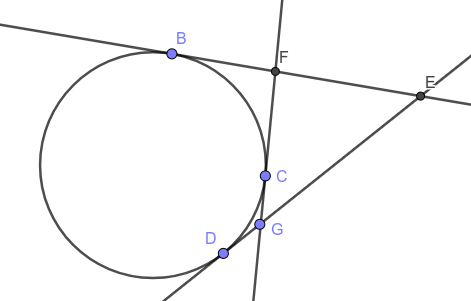
\includegraphics[width=0.4\textwidth]{cirtangents3}
            \end{center}
  \question
    \begin{parts}
      \part Find the area of the largest square that one can fit inside a circle of radius $ r $.
      \part Find the area of the smallest square that fits outside a circle of radius $ r $.
      \part Hence show that $ 2 < \pi < 4 $.
      \part How might you improve your estimate of $\pi $?
    \end{parts}
\end{questions}

\end{document}
